\documentclass [a4paper, 12pt]{article}

\usepackage{hyperref}
\usepackage{amssymb}
\usepackage{epsfig}
\usepackage{times}
\usepackage{float}
\usepackage[usenames,dvipsnames]{color}
\usepackage{ragged2e}
\usepackage[round,sort&compress]{natbib} 
\usepackage{multicol}
\usepackage{pgfgantt}
\usepackage[ddmmyyyy]{datetime}
\usepackage{textcomp}
\usepackage{pdflscape}
\usepackage[T1]{fontenc}

\setlength\columnsep{6cm}
\usepackage[top=2cm, bottom=2cm, left=2cm, right=2cm]{geometry}
\setlength{\headsep}{1cm}
\setlength{\footskip}{1cm}
\setlength{\parindent}{1cm}
\setlength{\bibsep}{-2pt}

\def\LCDM{\mbox{$\Lambda$CDM}}
\def\kms{\rm km\ s^{-1}}
\def\hkpc{\mbox{$\rm h^{-1}$kpc}}
\def\hMpc{\mbox{$\rm h^{-1}$Mpc}}
\def\hGpc{\mbox{$\rm h^{-1}$Gpc}}
\def\hMsun{\mbox{$\rm h^{-1}$M$_\odot$}}
\def\lesssim{_ <\atop{^\sim}}
\def\gtsim{_ >\atop{^\sim}}


\newcommand{\aladin}{{\textsc{A}{ladin}}}
\newcommand{\topcat}{{\textsc{Topcat}}}
\newcommand{\cassis}{{\textsc{Cassis}}}
\newcommand{\simbad}{{\textsc{SIMBAD}}}
\newcommand{\vizier}{{\textsc{v}izie\textsc{r}}}
\renewcommand{\dateseparator}{.}
\newcommand{\datatree}{\textsc{Data Tree}}

\begin{document}

\begin{center}
\includegraphics[width=0.3\textwidth]{../images/logo_euro.png} 
\hspace{5cm}
\includegraphics[width=0.4 
\textwidth]{../images/logo_asterics.png}\\
\vspace{1.5cm}
\begin{Huge} \textbf{ASTERICS - H2020 - 653477} \end{Huge} \end{center}

 
 \vspace{1cm}
\Huge
\begin{center}
\bf Discovery of brown dwarfs \\ mining the 2MASS and SDSS database
  \end{center}

 
\vspace{1cm}
\large
\begin{center}
Evolved from Tutorials lead by E. Solano and F. Jim\'enez-Esteban\\ %Giulia 
%Iafrate
\textit{Spanish Virtual Observatory}
\end{center}
\vspace{0.5cm}
\begin{center}
K. A. Lutz\\
\textit{updated with the new template for ASTERICS, new plots and for \aladin\ 
v10}
\end{center}
\vspace{0.5cm}
\begin{center}
last update \today
\end{center}


\vspace{3.5cm}
Template by Jenny G. Sorce


\newpage
\normalsize
\vfill
\tableofcontents
\vfill

\newpage

\justify
\section{Introduction}
Brown dwarfs are objects occupying the gap between the least massive
stars and the most massive planets. They are intrinsically faint objects so 
their detection is not straightforward and, in fact, was almost impossible 
until the advent of global surveys at deep optical and near-infrared bands like 
SDSS, 2MASS or DENIS among others. We propose here to mine the 2MASS point 
source catalogue (2MASS-PSC) and 
SDSS-DR9 databases to identify T-type brown dwarfs through an appropriate
combination of colours in the optical and the infrared, an approach that 
perfectly fits into the Virtual
Observatory.

\section{Goal of this tutorial} 
In this use case, we explore different ways to do the same tasks with different 
VO tools. These tasks include:
\begin{itemize}
\item obtaining data from the SDSS and 2MASS catalogues in a given sky region,
\item crossmatching the results of these searches,
\item filtering the resulting table for brown dwarfs, and 
\item verifying our sample of brown dwarfs.
\end{itemize}
\noindent Software packages needed for this tutorial are \aladin, \topcat\ and 
STILTS.

\section{\aladin}
Launch \aladin: Open a terminal and type: \texttt{java -jar Aladin.jar \&} \\

\noindent \textcolor{teal}{Discovery}: Search 2MASS-PSC and SDSS-DR9 sources 
around RA:~08h30m, DEC:~01d30m with a 14\,arcmin radius.
\begin{itemize}
    \item Enter the coordinates \texttt{08:30 01:30} in the \textbf{Command} 
    line of \aladin\ 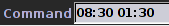
\includegraphics[width=0.2 
    \textwidth]{../images/aladin_command_coordinates.png} and press Enter.
    \item In the main viewing window the DSS colour image centred on the 
    entered coordinates appears. Zoom in and out by scrolling with your mouse 
    or by using the zoom register on the right hand side. Aim for a field of 
    view of approximately $14\times14$\,arcmin. Hint: the 
    cyan/blue numbers in the bottom of both the main viewing window and the 
    overview window in the bottom right corner of \aladin\ state the current 
    field of view. 
    \item Enter "2MASS PSC" in the \textbf{select} line 
    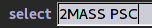
\includegraphics[width=0.17 
    \textwidth]{../images/aladin_select_2mass_psc.png} below the \datatree. 
    This will filter the entries in the \datatree\ to only show those that are 
    affiliated with the 2MASS point source catalogue. Note how some entries are 
    coloured in green and some in orange. This indicates whether a resource 
    has data available in the current field of view (green) or not (orange). 
    \item Choose the only green entry (\textbf{Catalog} $\rightarrow$ 
    \textbf{VizieR} $\rightarrow$ \textbf{II-Photometric Data} $\rightarrow$ 
    \textbf{2MASS-PSC...}) by clicking on it. In the pop-up window, make sure 
    to tick \textbf{in view} 
\includegraphics[width=0.1 
    \textwidth]{../images/aladin_load_inview.png} and \textbf{Load} the data 
    
\includegraphics[width=0.1 
    \textwidth]{../images/aladin_load_load.png} (see 
    Figure~\ref{fig:load_2mass_aladin}). This will load a catalogue of 
    approximately 1000 sources (\aladin\ will give you the number of rows of a 
    catalogue when hoovering over the entry of the catalogue in the stack on 
    the right of the main viewing window). You can change the appearance and 
    name of the data by selecting the plane "CDS/II/246/out" in the stack and 
    clicking the properties 
\includegraphics[width=0.03 
    \textwidth]{../images/aladin_button_properties.png} button. Alternatively 
    right-click on the plane and select \textbf{Properties...}. Rename the 
    plane to "2MASS-PSC".
    \begin{figure}[H]
        \center
        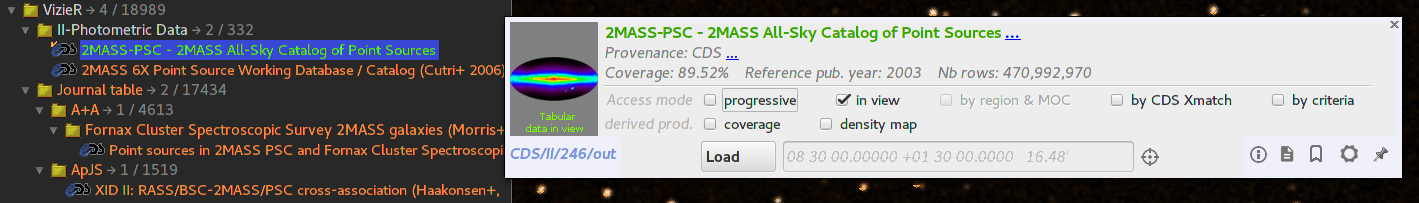
\includegraphics[width=0.6 
        \textwidth]{../images/aladin_load_2mass-pcs_cat.png}
        \caption{Loading the data available in the current field of view from 
        the 2MASS-PSC in \aladin.}
        \label{fig:load_2mass_aladin}
    \end{figure}
    \item Now we repeat the same steps for the SDSS-DR9 catalogue:
    \begin{itemize}
        \item Enter "SDSS DR9" in the \textbf{select} line.
        \item Choose the first green entry: \textbf{Catalog} $\rightarrow$ 
        \textbf{VizieR} $\rightarrow$ \textbf{V-Combined Data} $\rightarrow$ 
        \textbf{SDSS-DR9...}.
        \item \textbf{Load} the SDSS-DR9 catalogue data \textbf{in view}, which 
        will include of the order of 15,000 sources. Rename the new plane to 
        "SDSS-DR9".
    \end{itemize}
\end{itemize}
 
\noindent \textcolor{teal}{Crossmatching}: In this next step, we find common 
sources in 
the 2MASS-PSC and SDSS-DR9 catalogues. 
\begin{itemize}
    \item Open the \textbf{Catalog Cross-match tool} by either clicking the 
    cross-match button 
\includegraphics[width=0.03 
    \textwidth]{../images/aladin_button_crossmatch.png} or opening the menu 
    \textbf{Catalog} $\rightarrow$ \textbf{Cross match objects ...}. 
    \item In the \textbf{Catalog Cross-match tool} enter the two catalogues and 
    their coordinate columns, keep the default threshold for source separation 
    ($0 \le $ threshold $\le 4$) and select \textbf{Best matches} (see 
    Figure~\ref{fig:crossmatch_2mass_sdss_aladin}). Make sure 
    that the catalogue with the smaller number of sources is named in the first 
    line. Then hit \textbf{Perform cross-match}. A new plane called "XMatch" 
    will appear in the stack. It contains almost as many sources as the 
    2MASS-PSC plane. 
    \begin{figure}[H]
        \center
        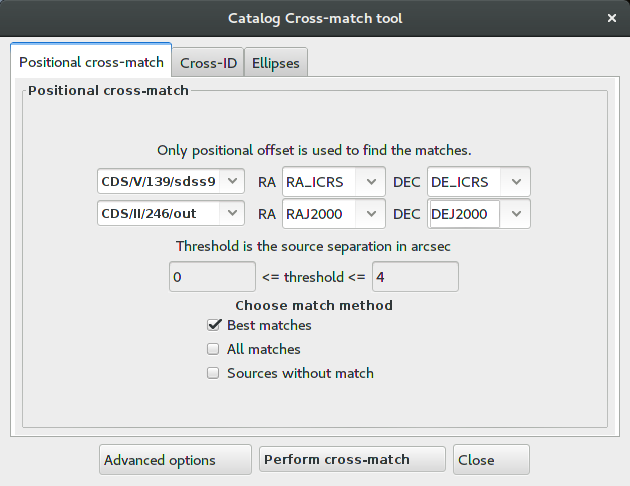
\includegraphics[width=0.5 
        \textwidth]{../images/aladin_crossmatch_sdss-2mass.png}
        \caption{Cross-matching 2MASS-PSC and SDSS DR9 in \aladin.}
        \label{fig:crossmatch_2mass_sdss_aladin}
    \end{figure}
\end{itemize}

\noindent \textcolor{teal}{Filtering}: Select those sources from our 
cross-match catalogue that are SDSS point sources and have characteristics that 
are expected from brown dwarfs. 
\begin{itemize}
    \item Hide the 2MASS-PSC and SDSS-DR9 planes by clicking on  
    
\includegraphics[width=0.06 
    \textwidth]{../images/aladin_button_table.png}. Note that moving the green 
    controller button in the bottom of this symbol changes the opacity of the 
    plane. 
    \item Select the XMatch plane by clicking on it. Open the \textbf{Filter 
    properties} window by either using the \textbf{Filter} button 
    
\includegraphics[width=0.04 
    \textwidth]{../images/aladin_button_filter.png} or following the menu 
    through \textbf{Catalog} $\rightarrow$ \textbf{Create a filter...}. 
    \item In the opened window \textbf{Properties of the filter} move to the 
    \textbf{Advanced mode} tab. Click on the 
\includegraphics[width=0.1 
    \textwidth]{../images/aladin_filter_columns.png} button and chose 
    \textbf{Columns in loaded catalogs...}. Select the "cl\_tab2" column from 
    the XMatch catalogue. 
    \item Complete the filter condition. It should be \texttt{\$\{cl\_tab2\}=6 
    \{draw\}}. This tells \aladin\, that only sources from the XMatch table 
    that adhere to the condition cl\_tab2=6 should be shown in the main viewing 
    window. The 
    \textbf{Actions}, \textbf{Maths...}, \textbf{Units} and \textbf{UCDs} 
    buttons next to the \textbf{Columns...} button further help in constructing 
    filter. 
    \item Click on 
\includegraphics[width=0.1 
    \textwidth]{../images/aladin_filter_apply.png}. This will apply the filter 
    to the XMatch plane. Clicking 
\includegraphics[width=0.1 
    \textwidth]{../images/aladin_filter_export.png} will create a new plane 
    "Filter.src", which only contains those sources from the XMatch plane that 
    comply with the filter criterion. Approximately 100 sources will be 
    excluded by this filtering action. 
\end{itemize}

Now that we have limited our sample to point sources according to the 
SDSS data, we move on to select brown dwarf candidates. Brown dwarfs are 
cool objects so they are not detected in the blue SDSS bands. We therefore 
select sources with no detection in the $u$ and $g$ SDSS bands \texttt{(u > 
22.0 \&\& g >22.2}. We furthermore search for sources fulfilling the brown 
dwarf criteria provided by Burgasser et al. (2000, ApJ, 531, L57): 
\texttt{((J-H)<0.3 \&\& (H-K)<0.3)}.

\begin{itemize}
    \item Hide the XMatch plane.
    \item Select the "Filter.src" plane. if you wish you can again change name 
    colour and plotting symbol by using the 
\includegraphics[width=0.03 
    \textwidth]{../images/aladin_button_properties.png} button.
    \item Repeat the same steps as for the previous filter. The filter 
    condition should now be: \texttt{\$\{umag\_tab2\} > 22.0 \&\& 
    \$\{gmag\_tab2\} > 22.2 \&\& \$\{Jmag\_tab1\} - \$\{Hmag\_tab1\} < 0.3 \&\&
    \$\{Hmag\_tab1\} - \$\{Kmag\_tab1\} < 0.3 \{draw\}}
    \item Click on 
\includegraphics[width=0.1 
    \textwidth]{../images/aladin_filter_apply.png}. Then click on 
    
\includegraphics[width=0.1 
    \textwidth]{../images/aladin_filter_export.png} to create a new plane with
    the filtered sources.
    \item A new plane "Filter.src$\sim$1" will be loaded in the \aladin\ main 
    window. It should contain 1 source. (RA\_2MASS:127.703265\,deg;
    DEC\_2MASS:1.475320\,deg). Note that the corresponding table column will be 
    shown when double-clicking on the source.
    \item If you have the \textbf{Simbad pointer} enabled (see 
    Figure~\ref{fig:simbadpointer_aladin}), hoover with the mouse over the 
    source until a small grey window appears. This grey window already tells 
    you the name (2MASS J08304878+0128311) and the object type (brownD*) of the 
    source. In order to visit the \simbad\ page for this source, click on the 
    name. 
    \begin{figure}[H]
        \center
        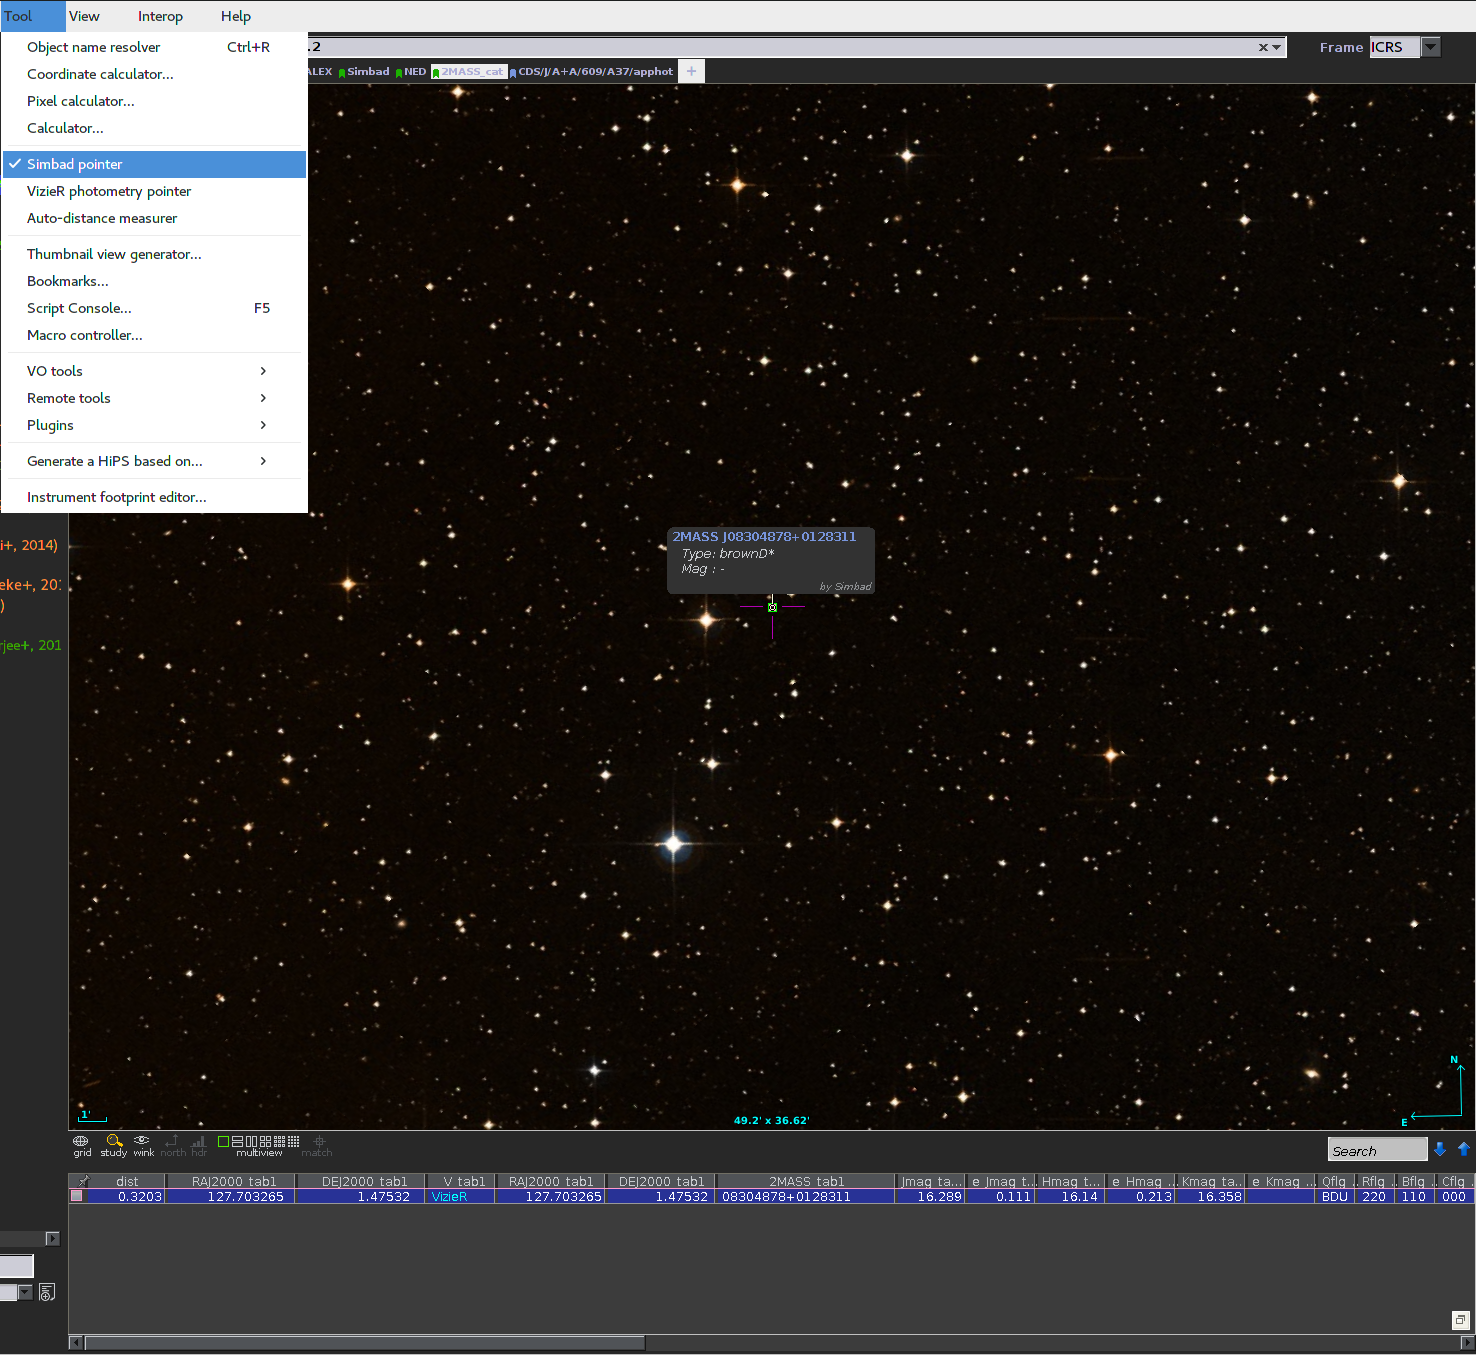
\includegraphics[width=0.75 
        \textwidth]{../images/aladin_simbad_pointer-brown_dwarf.png}
        \caption{Enabling the Simbad pointer in \aladin\ and getting basic 
        information on our resulting source. Hurray, it is indeed a brown 
        dwarf!}
        \label{fig:simbadpointer_aladin}
    \end{figure}
\end{itemize}

\section{\topcat}
Launch \topcat: Open a terminal and type: \texttt{java -jar topcat-full.jar \&} 
\\

\noindent \textcolor{teal}{Discovery}: Search 2MASS-PSC and SDSS-DR9 sources 
around RA:~08h30m, DEC:~01d30m with a 14\,arcmin radius.
\begin{itemize}
    \item In the \topcat\ main window follow the menu to \textbf{VO} 
    $\rightarrow$ \textbf{\vizier\ Catalogue Service}. A new window 
    (\textbf{\vizier\ Catalogue Service}) opens. 
    \item In this new window select \textbf{Cone Search} 
    
\includegraphics[width=0.2 
    \textwidth]{../images/topcat_vizier_cone-search.png} and enter the 
    coordinates, radius and units:\\
    RA: 08:30:00 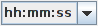
\includegraphics[width=0.1 
    \textwidth]{../images/topcat_vizier_hms.png}\\
    Dec: 01:30:00 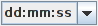
\includegraphics[width=0.1 
    \textwidth]{../images/topcat_vizier_dms.png}\\
    Radius: 14 
\includegraphics[width=0.1 
    \textwidth]{../images/topcat_vizier_arcmin.png}
    \item In the bottom half of the \textbf{\vizier\ Catalogue Service} window, 
    choose the \textbf{Surveys} tab, find and select "2MASS-PSC" and then click 
    OK. This will load the table "II\_246\_out" with 683 rows (i.\,e. sources) 
    in 
    the \topcat\ main window. 
    \item Repeat the previous steps for SDSS-DR9. This will load the table 
    "V\_139\_SDSS9" with 12,404 sources into the \topcat\ main window. 
    \item Alternatively, you could broadcast the 2MASS and SDSS DR9 catalogs 
    from \aladin\ to \topcat\ using SAMP (Simple Application Messaging 
    Protocol): In \aladin, right-click on the "2MASS-PSC" plane in the stack. 
    Then select \textbf{Broadcast selected tables to ...} $\rightarrow$ 
    \textbf{topcat} (see Figure~\ref{fig:broadcast_aladin_topcat}). The table 
    should appear in the \topcat\ main window. Use 
    the same approach for the SDSS DR9 sources.
    \begin{figure}[H]
        \center
        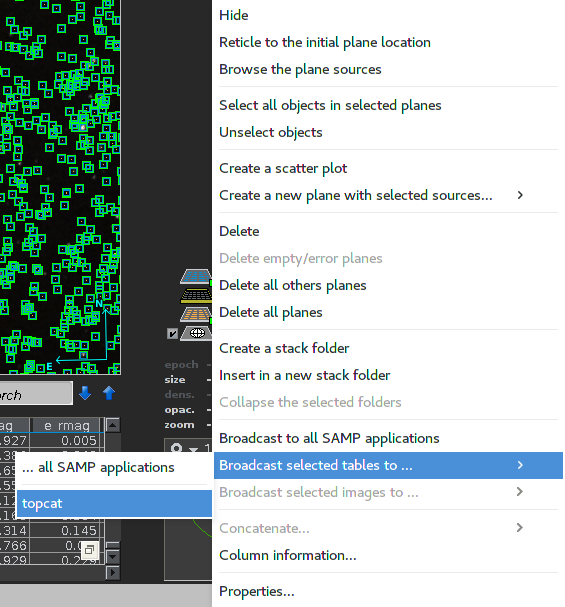
\includegraphics[width=0.75 
        \textwidth]{../images/aladin_send_table_topcat.png}
        \caption{Broadcasting a table from \aladin\ to \topcat\ via SAMP. }
        \label{fig:broadcast_aladin_topcat}
    \end{figure}
\end{itemize}

\noindent \textcolor{teal}{Crossmatching}: In this next step, we find common 
sources in the 2MASS-PSC and SDSS-DR9 catalogues. 
\begin{itemize}
    \item Open the \topcat\ \textbf{Match Tables} window by either following 
    the menu in the main window to \textbf{Joins} $\rightarrow$ \textbf{Pair 
    Match} or simply using the 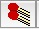
\includegraphics[width=0.04 
    \textwidth]{../images/topcat_button_xmatch.jpg} button. 
    \item In the \textbf{Match Tables} window set the following parameters (see 
    Figure~\ref{fig:crossmatch_topcat}):
    \begin{itemize}
        \item In the Match criteria box:\\
        Algorithm: Sky\\
        Max error: 4\,arcsec
        \item Table1: II\_246\_out (2MASS-PSC). RA/Dec columns: RAJ2000,
        DEJ2000.
        \item Table2: V\_139\_sdss9 (SDSS-DR9). RA/Dec columns: RA\_ICRS,
        DE\_ICRS.
        \item Output Rows box:\\
        Match selection: Best match, symmetric\\
        Join Type: 1 and 2
    \end{itemize}
    Then click \textbf{Go}, get the notification that 679 pairs were found and 
    confirm that a new plane "match(1,2)" with 679 sources is loaded.
    \begin{figure}[H]
        \center
        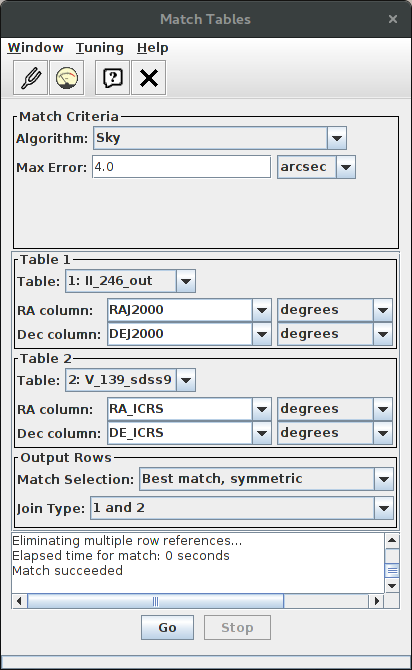
\includegraphics[width=0.4 
        \textwidth]{../images/topcat_match_2MASS_SDSS.png}
        \caption{Cross-matching the 2MASS PSC and the SDSS DR9 tables in 
        \topcat. }
        \label{fig:crossmatch_topcat}
    \end{figure}
\end{itemize}

\noindent \textcolor{teal}{Filtering}: Select those sources from our 
cross-match catalogue that are SDSS point sources and have characteristics that 
are expected from brown dwarfs. 
\begin{itemize}
    \item Again, we first remove all sources that not SDSS point sources. To do 
    so select the "match(1,2)" table and then open the \topcat\ subset window 
    by either following the menu in the main 
    window to \textbf{Views} $\rightarrow$ \textbf{Rows Subsets} or use the 
    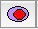
\includegraphics[width=0.04 
    \textwidth]{../images/topcat_button_subset.jpg} button. 
    \item In the newly opened window \textbf{Row Subsets} create a new subset 
    by clicking 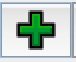
\includegraphics[width=0.04 
    \textwidth]{../images/topcat_button_add.jpg}. 
    \item In the new \textbf{Define Row Subset} window fill in the form with:\\
    Subset Name: filt1\\
    Expression: \texttt{cl==6} or \texttt{\$24==6}. The second option is 
    particularly useful when two columns have the same name except for upper 
    and lower case e.\,g. one named "cl" and another one "CL", because \topcat\ 
    expression are case insensitive. You can find the number of a column in the 
    table metadata, accessible via 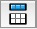
\includegraphics[width=0.04 
    \textwidth]{../images/topcat_button_metadata.jpg}. 
    \item Click \textbf{OK}. In the \textbf{Current Table Properties} panel in 
    the main window, you can now select in the \textbf{Row Subset} dropdown 
    menu between \textbf{All} or \textbf{filt1}. If you chose \textbf{filt1}, 
    649 sources are included in the table. 
    \item Before we move on, let's have a look at the content of the new table. 
    To do so click 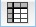
\includegraphics[width=0.04 
    \textwidth]{../images/topcat_button_open-tab.jpg}. This will open a new 
    window within 
    which you can scroll through the table. 
    \item In order to implement the brown dwarf selection criteria, we have two 
    options:
    \begin{itemize}
        \item Go back to the \textbf{Row Subset} window of the match(1,2) table 
        (which table the window is working on is mentioned in the line below 
        the buttons). Add a second subset 
        with (see Figure~\ref{fig:filtering_topcat}):\\
        Subset Name: filt2\\
        Expression: \texttt{cl==6 \&\& umag>22.0 \&\& gmag> 22.2 \&\& 
        Jmag-Hmag<0.3 \&\& Hmag-Kmag<0.3}\\
        \item Select the match(1,2) table and for \textbf{Row Subset}  
        \textbf{filt1}. Then duplicate the table by following the menu to 
        \textbf{File} $\rightarrow$ \textbf{Duplicate Table}. This will create 
        a new table called "Copy of 3" that only includes the rows of the filt1 
        subset. Now we can create a new subset of this table by first selecting 
        it in the main window, then opening the \textbf{Row Subsets} window 
        with 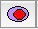
\includegraphics[width=0.04        
        \textwidth]{../images/topcat_button_subset.jpg} and adding a new subset 
        with 
        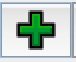
\includegraphics[width=0.04 
        \textwidth]{../images/topcat_button_add.jpg}. The Expression would be 
        \texttt{umag>22.0 \&\& gmag> 22.2 \&\& Jmag-Hmag<0.3 \&\& 
        Hmag-Kmag<0.3}. 
    \end{itemize} 
    The second option might appear a bit cumbersome but will come in handy for 
    more complex analyses. Either way, after the filtering process only one 
    source remains: RA:127.703265\,deg; DEC:1.475320\,deg. 
    \begin{figure}[H]
        \center
        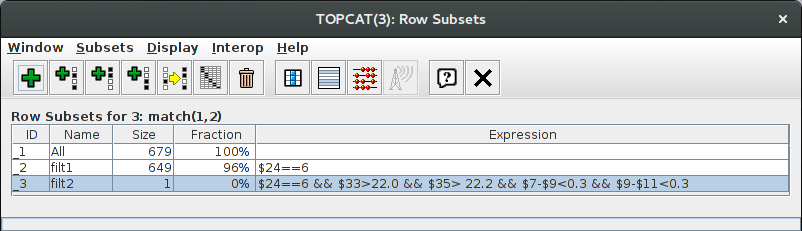
\includegraphics[width=0.8 
        \textwidth]{../images/topcat_filter_2MASS_SDSS.png}
        \caption{Subset of the cross-matched 2MASS PSC/ SDSS DR9 tables in 
            \topcat. }
        \label{fig:filtering_topcat}
    \end{figure}
    \item In order to visualise the source and check whether it is indeed a 
    brown dwarf, you could now broadcast the filtered table to \aladin\ (if 
    \aladin\ is running):
    \begin{itemize}
        \item In the \topcat\ main window select the match(1,2) table and filt2 
        as the row subset. 
        \item Now either click the broadcast button 
        
\includegraphics[width=0.04        
        \textwidth]{../images/topcat_button_broadcast.jpg} or go through the 
        menu 
        \textbf{Interop} $\rightarrow$ \textbf{Send table to... } $\rightarrow$ 
        \textbf{Aladin}. 
        \item Now a new table should appear in the \aladin\ stack and you can 
        proceed as before. 
    \end{itemize}
\end{itemize}

\section{Advanced Scripting in \aladin}
\aladin\ has a script mode to build a list of commands to be processed. The 
workflow can be executed automatically for a list of targets. If you closed 
\aladin\, launch it again (\texttt{java -jar Aladin.jar \&}). If \aladin\ 
is open, click on any plane, click right mouse button and select "Delete all 
planes" (to clean up a little bit before we move on). 
\newpage
\begin{itemize}
    
\item Before we get started in \aladin, we create two text files in any text 
editor and save them. The content of the script file looks as follows:\\

\texttt{2mass = get VizieR(2MASS-PSC) \$1 \$2 14\textquotesingle}\\
\texttt{sync}\\
\texttt{sdss = get VizieR(SDSS-DR9) \$1 \$2 14\textquotesingle}\\
\verb|sync|\\
\verb|2massdss= xmatch 2mass sdss 4 bestmatch|\\
\verb|sync|\\
\verb|hide 2mass|\\
\verb|sync|\\
\verb|hide sdss|\\
\verb|sync|\\
\verb|filter candidates { ${cl_tab2}==6 && ${umag_tab2}>22.0 && |\\
\verb|    ${gmag_tab2}>22.2 && ${Jmag_tab1}-${Hmag_tab1}<0.3 &&|\\
\verb|    ${Hmag_tab1}-${Kmag_tab1}<0.3 {draw} }|\\
\verb|#(the 3 lines above are 1 single line, remove the tabs and linebreaks)|\\
\verb|sync|\\
\verb|select 2massdss|\\
\verb|sync|\\
\verb|cplane candidates|\\

The parameter file looks like this:
\begin{verbatim}
# RA DEC
08:30:00, 01:30:00
\end{verbatim}

\item Now go back to the \aladin\ main window and open an \textbf{Macros} 
window by using the menu \textbf{Tool} $\rightarrow$ \textbf{Macro 
controller...}. 
\item In the \textbf{Macros} window use the menu to load the script file: go to 
\textbf{File} $\rightarrow$ \textbf{Load script} or type CTRL+S. Select and 
open your script file from where you saved it before. 
\item Now do the same for the parameter file: go to 
\textbf{File} $\rightarrow$ \textbf{Load params} or type CTRL+P. Select and 
open your parameter file from where you saved it before. 
\item Select the coordinate by clicking on their entry in the \textbf{Macros} 
window and push \textbf{Exec. current params} 

\includegraphics[width=0.15        
\textwidth]{../images/aladin_macros_execcurrent.png}. \aladin\ will now go 
through the script executing the steps we took before by itself. Once \aladin\ 
is finished you should see one source highlighted on the screen, which is again 
the brown dwarf we identified before. 
\end{itemize}
More information on how to build scripts in \aladin\ can be found in the 
\aladin\ menu at: \textbf{Help} $\rightarrow$ \textbf{Help on script commands} 
or by using CTRL+F5. 

\section{STILTS}
STILTS has the same underlying library as \topcat\ but is a command-line tool 
and can thus be scripted. 
\begin{itemize}
    \item Copy the file "stilts.script" 
    (\url{http://cds.unistra.fr/tutorials/CDS-tutorial/stilts.script}) to your 
    local computer. You may also use the version further below. For the version 
    below, be aware that line-breaks had to be inserted to be able to fit the 
    commands on an A4 page. Make sure that you remove all line-breaks, for 
    which the old line does not end with a "\verb|\|" and the new line has an 
    extra large indent (i.\,e. all line-breaks that are within a string, an 
    URL, ...). 
    Leave no blank spaces, where you remove these line-breaks.
    \item Make the script executable by typing \texttt{chmod u+x stilts.script} 
    into a command line.
    \item Execute it by entering \texttt{./stilts.script} into a command 
    line. A new file ("candidate.xml") is created. It contains the same single 
    object found in the previous workflows.
\end{itemize}

%\newpage
The commands included in the STILTS script to find the brown dwarf:\\
\begin{small}
\noindent\verb|java -jar /path/to/stilts/stilts.jar tpipe \| \\
\verb|    |
\textquotesingle
\verb|in=http://vizier.u-strasbg.fr/viz-bin/conesearch/II/246?| \\
\verb|        -out.max=unlimited&verb=3&RA=127.5&DEC=+1.5&SR=0.2333333|
\textquotesingle
\verb| \|\\
\verb|    out=2mass.xml| \\

\noindent\verb|java -jar /path/to/stilts/stilts.jar tpipe \| \\
\verb|    |
\textquotesingle
\verb|in=http://vizier.u-strasbg.fr/viz-bin/conesearch/V/139?| \\
\verb|        -out.max=unlimited&verb=3&RA=127.5&DEC=+1.5&SR=0.2333333|
\textquotesingle
\verb| \| \\
\verb|    out=sdssdr9.xml| \\

\noindent\verb|java -jar /path/to/stilts/stilts.jar tskymatch2 ifmt1=votable |
\verb|in1=2mass.xml \| \\
\verb|    ifmt2=votable in2=sdssdr9.xml ra1=RAJ2000 dec1=DEJ2000 |
\verb|ra2=RA_ICRS \| \\
\verb|    dec2=DE_ICRS error=4 find=best join=1and2 ofmt=votable |
\verb|out=cross.xml| \\

\noindent\verb|java -jar /path/to/stilts/stilts.jar tpipe ifmt=votable | 
\verb|in=cross.xml \| \\
\verb|    cmd=|\textquotesingle
\verb|select |
\verb|"cl==6 && umag>22.0 && gmag>22.2 && |\\
\verb|        Jmag-Hmag<0.3 && Hmag-Kmag<0.3"|
\textquotesingle
\verb| \| \\
\verb|    ofmt=votable out=candidate.xml| \\
\end{small}

%\bibliographystyle{unsrtnat} % Use the "unsrtnat" BibTeX style for formatting the Bibliography
%\bibliography{Bibliography}


\end{document}


